\section{Matrix-Vector Multiplication}
\label{sec:spmv}

In this section we model abstract matrix-vector multiplication and CSR sparse-matrix vector multiplication (SpMV) and demonstrate the refinement check needed to verify its correctness.

\begin{figure}
\begin{subfigure}[b]{0.5\textwidth}
  \centering
  \begin{tikzpicture}

\matrix (A) [
  matrix of math nodes,
  row sep=.5ex,
  column sep=.5ex,
  left delimiter={[},right delimiter={]},
  nodes={text width=1.5em, text height=1.5ex, text depth=.5ex, align=center}
]
{
  A_{00} & A_{01} & A_{02} \\
  A_{10} & A_{11} & A_{12} \\
  A_{20} & A_{21} & A_{22} \\
};

\node (times) [right=0.75em of A] {$\times$};

\matrix (x) [
  matrix of math nodes,
  left delimiter=\{,
  right delimiter=\},
  row sep=.5ex,
  nodes={text height=1.5ex, text depth=.5ex,}, 
  right=of A
] {
  x_0\\
  x_1\\
  x_2\\
};

\node (eq) [right=1em of x] {$=$};

\matrix (b) [
  matrix of math nodes,
  left delimiter=\{,
  right delimiter=\},
  row sep=.5ex,
  nodes={text height=1.5ex, text depth=.5ex},
  right=1em of eq
] {
  \bm{A_0 \cdot x_0}\\
  A_1 \bm{\cdot} x_1\\
  A_2 \bm{\cdot} x_2\\
};

\end{tikzpicture}
  \caption{}
  \label{fig:mvm}
\end{subfigure}
{\color{lightgray}\rule{0.4\textwidth}{0.1pt}}
\par\bigskip
\begin{subfigure}[b]{0.5\textwidth}
  \centering
  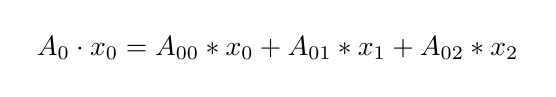
\begin{tikzpicture}
\node (A0x0) {
  $\bm{A_0 \cdot x_0} = A_{00}*x_0 + A_{01}*x_1 + A_{02}*x_2$ 
};
\end{tikzpicture}
  \caption{}
  \label{fig:dp}
\end{subfigure}
{\color{lightgray}\rule{0.4\textwidth}{0.1pt}}
\par\bigskip
\begin{subfigure}[b]{0.5\textwidth}
  \centering
  \begin{myquote}
\Bsig SumProd \Bextends Value \{\\
\TA values: \Bint\\
\TB $\rightarrow$ \Blone (Value-SumProd)\\
\TB $\rightarrow$ (Value-SumProd)\\
\} \{\\
\TA \Ball i: values.\Buniv.\Buniv\ $|$ i $\geq$ 0\\
\}
\end{myquote}
  \caption{}
  \label{fig:dpt}
\end{subfigure}
\caption{(\subref{fig:mvm}) a matrix-vector multiplication, (\subref{fig:dp}) the components of the first dot product in (\subref{fig:mvm}), and (\subref{fig:dpt}) the relational form of the same dot product.}
\end{figure}

The result of the matrix-vector multiplication $\bm{A}x = b$ is a densely populated vector, $y$, in which each value is the dot product of a single row of the matrix $A$ with the vector $x$.  A dot product is simply a sum of products in which each product is of two values located at the same index within two vectors, as shown in ~\figurename~\ref{fig:dp}.

\begin{figure}
\lstinputlisting[language=alloy]{models/sumprod.als}
\caption{SumProd Signature}
\label{model:sumprod}
\end{figure}

In order to compare the result of an abstract matrix-vector multiplication with the result of a concrete one, we must be able to compare arrays of dot products.  Rather than compare numerical values, we wish to compare the vectors dot products as a composition of the values.  To do so we introduce the \texttt{SumProd} signature, shown in \figurename~\ref{model:sumprod}.  To represent a sum of products, \texttt{SumProd} contains a single field, \texttt{values}, that maps unique integers to \texttt{Value} pairs. Through this field, the \texttt{SumProd} signature is able to represent a sum of products as a table in which each row contains a product of two values, and the summation is composed of all rows, as shown in \figurename~\ref{fig:dpt}.  Additionally, the integer value associated with each row indicates the index from which the values in that row originate.  To represent the vectors $b$ and $x$ in the matrix-vector multiplication $\bm{A}x = b$, we use a sequence of \texttt{SumProd}s and a sequence of \texttt{Value}s, respectively.

\begin{figure}
\lstinputlisting[language=alloy]{models/mvm.als}
\caption{Matrix-Vector Multiplication for Abstract and CSR.}
\label{model:mvm}
\end{figure}

The matrix-vector multiplication models for both the abstract and CSR format are found in \figurename~\ref{model:mvm}.  In both cases, the dimensions of the matrix and vectors are tested for compatibility in a matrix-vector multiplication, and dot products are generated for the solution in a row-wise fashion.  Note that the \texttt{dotProd} predicate does not include products that will evaluate to zero in the resulting SumProd.  As such, the dot products will be equivalent regardless of whether the vector originates from a dense or sparse representation.  Further note that the same \texttt{dotProd} predicate is used in both the abstract and CSR cases.  This is enabled by the \texttt{getrow} helper function which extract sets of column$\rightarrow$value pairs in a row-wise fashion from a CSR matrix.

The refinement check is performed by the \texttt{refines} predicate.  Alloy has shown this refinement to be correct for matrices up to $5\times5$ with 10 unique values.

The nature of the refinement check here is similar to the square diagram above, but need to show it precisely as it varies slightly.

This same method of data refinement has been used to model SpMV for the ELL format as well.